% !TEX encoding = UTF-8 Unicode
% !TEX TS-program = pdflatexshell

\documentclass[../main/main.tex]{subfiles}

\begin{document}
%\setcounter{chapter}{1}
%\setcounter{section}{1}
\section{Homework}

Entrega del problema 2.12 y 2.16: 28 de octubre



\subsection*{Problem 2.12}
\emph{Encontrar la señal analítica asociada a la función $\cos x +\sin x$}.


I am not sure what it means by ``find the analytical signal of the function''. However, since this is a Radon equation problem, I imagine we mean that, that is the Radon signal $R(s, \alpha) = \ddelta{s-\cos \alpha} + \ddelta{s-\sin \alpha}$ and we need to find the actual mass density, or $R(s, \alpha) = \ddelta{s-\cos \alpha - \sin\alpha}$

If we understand it as $R(s, \alpha) = \ddelta{s-\cos \alpha} + \ddelta{s-\sin \alpha}$

% modifying example from p.345 from the Tikz & PGF Manual for Version 3.1.8b
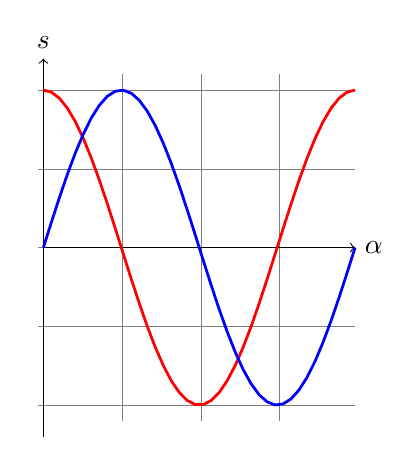
\begin{tikzpicture}[domain=0:2*pi, samples=40, y=2 cm, x =0.63cm]
\draw[very thin,color=gray] (-0.1,-1.1) grid ({2*pi},1.1);
  \draw[->] (0,0) -- (2*pi,0) node[right] {$\alpha$};
  \draw[->] (0,-1.2) -- (0,1.2) node[above] {$s$};
\draw[color=red, line width=1pt] plot (\x,{cos(\x r)}) node[right] {};
\draw[color=blue, line width=1pt] plot (\x,{sin(\x r)}) node[right] {};
\end{tikzpicture}
\qquad
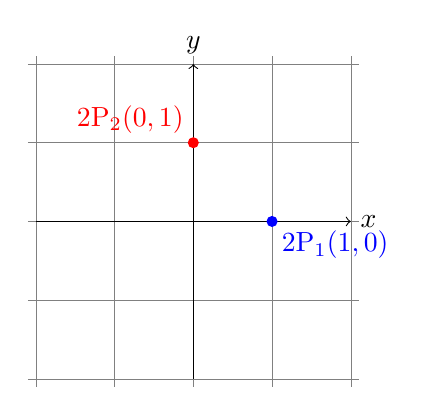
\begin{tikzpicture}[x=1cm, y=1cm]
	\draw[very thin,color=gray] (-2.1,-2.1) grid (2.1,2.1);
	\draw[->] (-2,0) -- (2,0) node[right] {$x$};
	\draw[->] (0,-2) -- (0,2) node[above] {$y$};
    \fill[color=blue] (1, 0) circle [color=blue, radius=2pt]
    	node[anchor=north west]{$2\textrm{P}_{1}(1, 0)$};
    \fill[color=red] (0, 1) circle [color=red, radius=2pt]
    	node[anchor=south east]{$2\textrm{P}_{2}(0,1)$};
\end{tikzpicture}

If we instead understand it as $R(s, \alpha) = \ddelta{s-\cos \alpha-\sin \alpha} = \ddelta{s-\sqrt{2} \cos(\pi/4-x)}=$

% modifying example from p.345 from the Tikz & PGF Manual for Version 3.1.8b
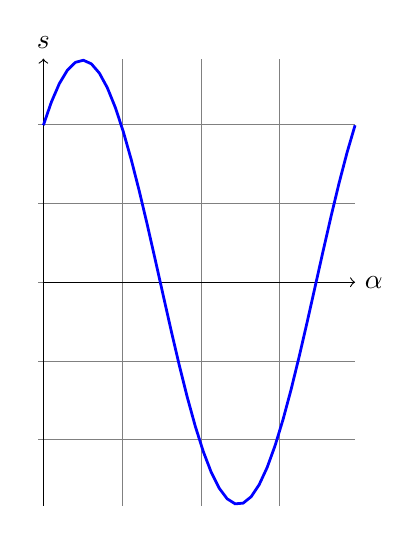
\begin{tikzpicture}[domain=0:2*pi, samples=40, y=2 cm, x =0.63cm]
\draw[very thin,color=gray] (-0.1,-1.42) grid ({2*pi},1.42);
  \draw[->] (0,0) -- (2*pi,0) node[right] {$\alpha$};
  \draw[->] (0,-1.42) -- (0,1.42) node[above] {$s$};
\draw[color=blue, line width=1pt] plot (\x,{1.41*cos(\x r-pi/4 r)}) node[right] {};
\end{tikzpicture}
\qquad
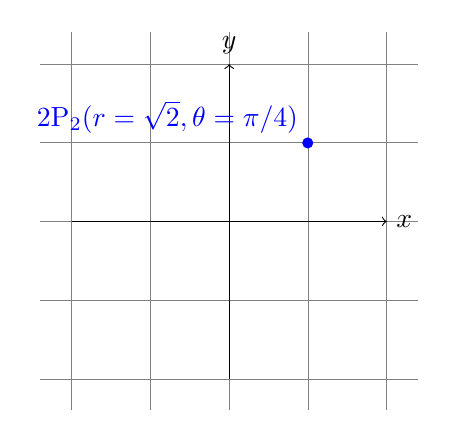
\begin{tikzpicture}[x=1cm, y=1cm]
	\draw[very thin,color=gray] (-2.4,-2.4) grid (2.4,2.4);
	\draw[->] (-2,0) -- (2,0) node[right] {$x$};
	\draw[->] (0,-2) -- (0,2) node[above] {$y$};
    \fill[color=blue] (45:1.41) circle [color=red, radius=2pt]
    	node[anchor=south east]{$2\textrm{P}_{2}(r=\sqrt{2},\theta=\pi/4)$};
\end{tikzpicture}

\subsection*{Problema 2.16}

\emph{Presentar esquemáticamente la transformada de Radon (senograma) de la señal}
\begin{equation*}
	f(x,y) =
	\sqrt{2}
	\ddelta{x - \frac 1 {\sqrt{2}}}
	\ddelta{\sqrt{2}y - 1}
	+ 2
	\ddelta{x-1}
	\ddelta{y}.
\end{equation*}

Firstly, we can re-write that equation as

 \begin{align*}
 	f(x,y) &=
 	\sqrt{2}
 	\ddelta {x - \frac 1 {\sqrt{2}}}
 	\ddelta {\sqrt{2}\left(y - \frac 1 {\sqrt{2}}\right)}
 	+ 2
 	\ddelta{x-1}
 	\ddelta{y} \\
 	&=
 	\ddelta {x - \frac 1 {\sqrt{2}}}
 	\ddelta {y - \frac 1 {\sqrt{2}}}
 	+ 2
 	\ddelta{x-1}
 	\ddelta{y}.
 \end{align*}

Where we have used that $\ddelta {ax} = \frac 1 {\abs{a}} \ddelta{x}$
Therefore, this 2-D delta function is representing two isolated points. In a sketch, we could say it is somewhat like

\begin{equation*}
	f(x,y) = 2 \textrm{P}_{1}(1, 0) + \textrm{P}_{2}\left(\frac 1 {\sqrt{2}}, \frac 1 {\sqrt{2}}\right).
\end{equation*}

	      \begin{center}

		      \begin{tikzpicture}[x=1cm, y=1cm]
			      % grid
			      \draw[help lines, dotted] (-2.5,-2.5) grid (2.5, 2.5);
			      \draw[thin, dotted](-2.5,0)--(2.5,0) node[anchor=south east]{$x$};
			      \draw[thin, dotted](0,-2.5)--(0,2.5) node[anchor=north west]{$y$};
			      \fill (1, 0) circle [radius=2pt]
			      	node[anchor=north west]{$2\textrm{P}_{1}(1, 0)$};
			      \fill (1/1.414, 1/1.414) circle [radius=2.82pt]
			      	node[anchor=south east]{$2\textrm{P}_{2}\left(\frac 1 {\sqrt{2}}, \frac 1 {\sqrt{2}}\right)$};


		      \end{tikzpicture}
	      \end{center}


The radon transformation is a linear transformation, and a point gets converted to the curved line

\begin{equation*}
s(\alpha) = r_{0}\cos(\alpha_{0}- \alpha).
\end{equation*}


In our formula we get $r_{1} = r_{2}=1$ and $\alpha_{1} = 0$ $\alpha_{2}=\pi/4$ and we therefore obtain the 2-D Radon map that follows
\nopagebreak

% modifying example from p.345 from the Tikz & PGF Manual for Version 3.1.8b
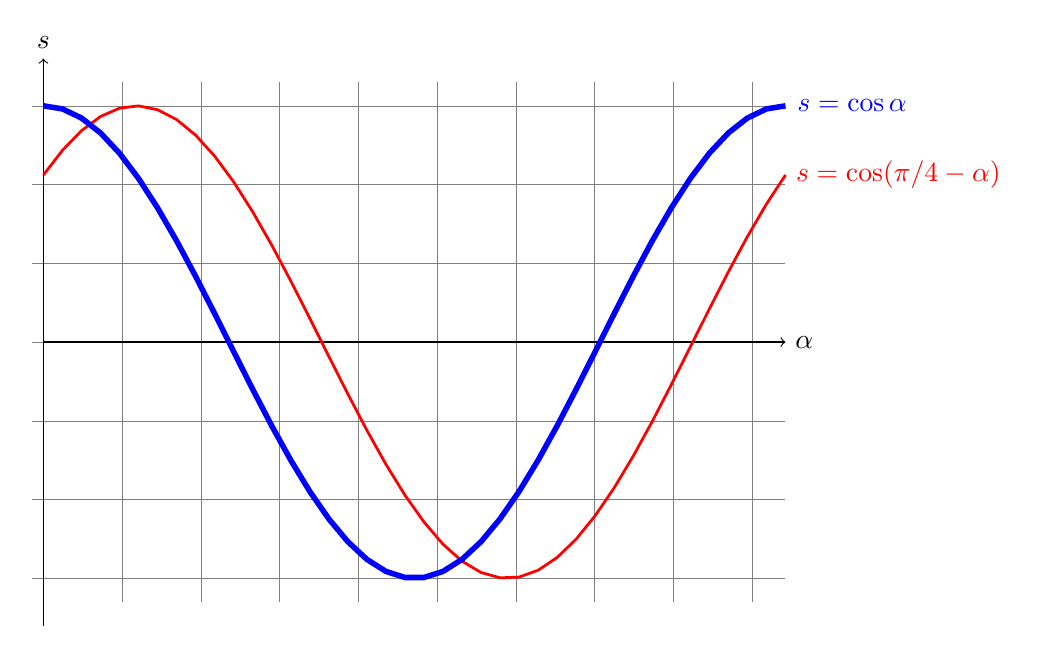
\begin{tikzpicture}[domain=0:2*pi, samples=40, x=1.5cm, y=3cm]
\draw[very thin,color=gray] (-0.1,-1.1) grid ({2*pi},1.1);
  \draw[->] (0,0) -- (2*pi,0) node[right] {$\alpha$};
  \draw[->] (0,-1.2) -- (0,1.2) node[above] {$s$};
\draw[color=red, line width=1pt] plot (\x,{cos(pi/4 r-\x r)}) node[right] {$s = \cos(\pi/4 - \alpha)$};
\draw[color=blue, line width=2pt] plot (\x,{cos(\x r)}) node[right] {$s = \cos \alpha$};
\end{tikzpicture}
\end{document}
